

\includegraphics[height=1.5cm]{images/pictograms/benchmark}

\lstinputlisting[language=bash,basicstyle=\small]{python_codes/fieldstone_07/keywords.ascii}

\begin{center}
\inpython
{\small Code: \url{https://github.com/cedrict/fieldstone/tree/master/python_codes/fieldstone_07}}
\end{center}

\par\noindent\rule{\textwidth}{0.4pt}
%%%%%%%%%%%%%%%%%%%%%%%%%%%%%%%%%%%%%%%%%%%%%%%%%%%%%%%%%%%%%%%%%%%%%%%%%%%%%%%%%%%%%%%%%

Following SolCx and SolKz, the SolVi inclusion benchmark solves 
a problem with a discontinuous viscosity field, but in this case 
the viscosity field is chosen in such a way that the discontinuity 
is along a circle. Given the regular nature of the grid used by a majority of codes and the present one, 
this ensures that the discontinuity in the viscosity never aligns to cell boundaries.
This in turns leads to almost discontinuous pressures along the interface which are difficult to represent accurately.
Schmid \& Podlachikov (2003) \cite{scpo03} derived a simple analytic solution for the pressure and 
velocity fields for a circular 
inclusion under simple shear and it was used in \cite{deka08,sunh10,dumg11,krhb12,gemd13}.

Because of the symmetry of the problem, we only have to solve over the top right quarter of the domain.
The analytical solution requires a strain rate boundary condition (e.g., pure shear) to be applied far away 
from the inclusion. In order to avoid using very large domains and/or dealing with this type of boundary condition 
altogether, the analytical solution is evaluated and imposed on the boundaries of the domain. 
By doing so, the truncation error introduced while discretizing the strain rate boundary condition is removed.

A characteristic of the analytic solution is that the pressure is zero inside the inclusion, while outside it follows the relation
\begin{equation}
p_m = 4 \dot{\epsilon}
\frac{\eta_m(\eta_i-\eta_m)}{\eta_i+\eta_m}
\frac{r_i^2}{r^2} \cos(2\theta)
\end{equation}
where $\eta_i = 10^3$ is the viscosity of the inclusion 
and $\eta_m = 1$ is the viscosity of the background media, $\theta=\tan^{-1}(y/x)$,
and $\dot{\epsilon}=1$ is the applied strain rate.

Deubelbeiss \& Kauss (2008) \cite{deka08} thoroughly investigated this problem with various 
numerical methods (FEM, FDM), with and without tracers, 
and conclusively showed how various averagings lead to different results. 
Duretz et al (2011) \cite{dumg11} obtained a first order convergence for both pressure and velocity, 
while Kronbichler et al (2012) \cite{krhb12}
and Gerya et al (2013) \cite{gemd13} showed that the use of adaptive mesh refinement in respectively the FEM and FDM 
yields convergence rates which depend on refinement strategies. 

\begin{center}
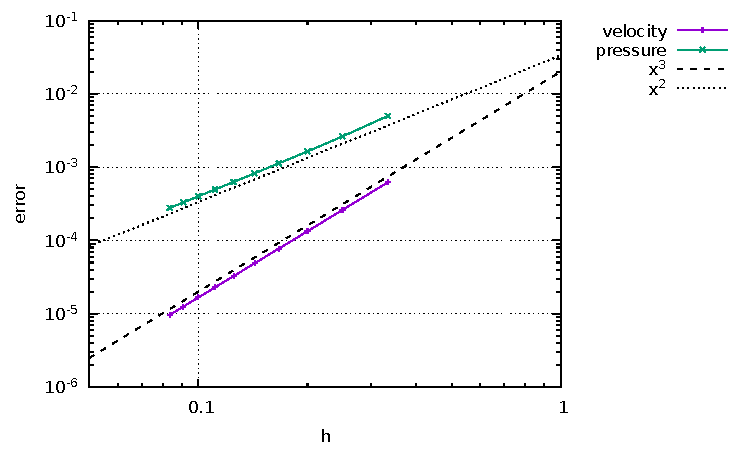
\includegraphics[width=8cm]{python_codes/fieldstone_07/results/errors}\\
{\captionfont Velocity and pressure error convergence as a function of mesh size.}
\end{center}

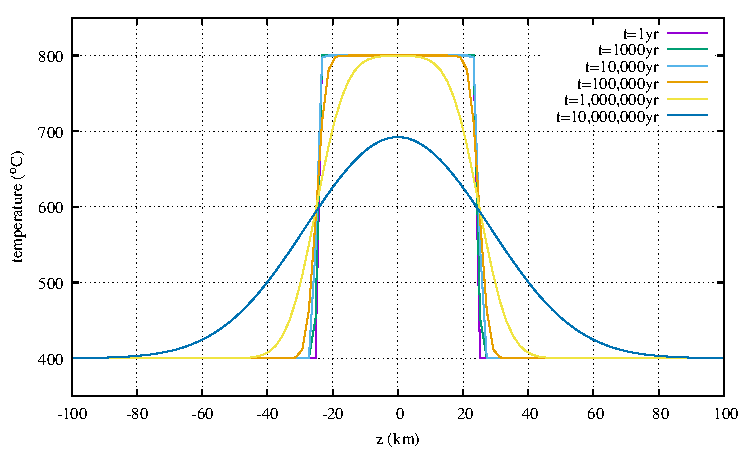
\includegraphics[width=16cm]{python_codes/fieldstone_07/results/solution}

\begin{center}
\includegraphics[width=7cm]{python_codes/fieldstone_07/results/pressbottom}
\includegraphics[width=7cm]{python_codes/fieldstone_07/results/veldiag}\\
{\captionfont Left: Pressure at the bottom of the domain. Right: $u$ on the diagonal $x=y$.}
\end{center}

